\section{The Composable Stack}

Composable's vision is to create a protocol that allows for communication cross-ecosystem. The result is a Port Control Protocol like system for blockchains.
%
The architecture - the tech stack will be covered in the following sections.

The end result is multifaceted; users can perform cross-chain actions, and the overarching blockchain ecosystem is repositioned as a network of agnostic liquidity and available yield. Throughout this experience, Composable allows users to tailor their experience to maximize for a desired parameter while minimizing ecosystem-specific decision making.

%
\begin{figure}
    \centering
    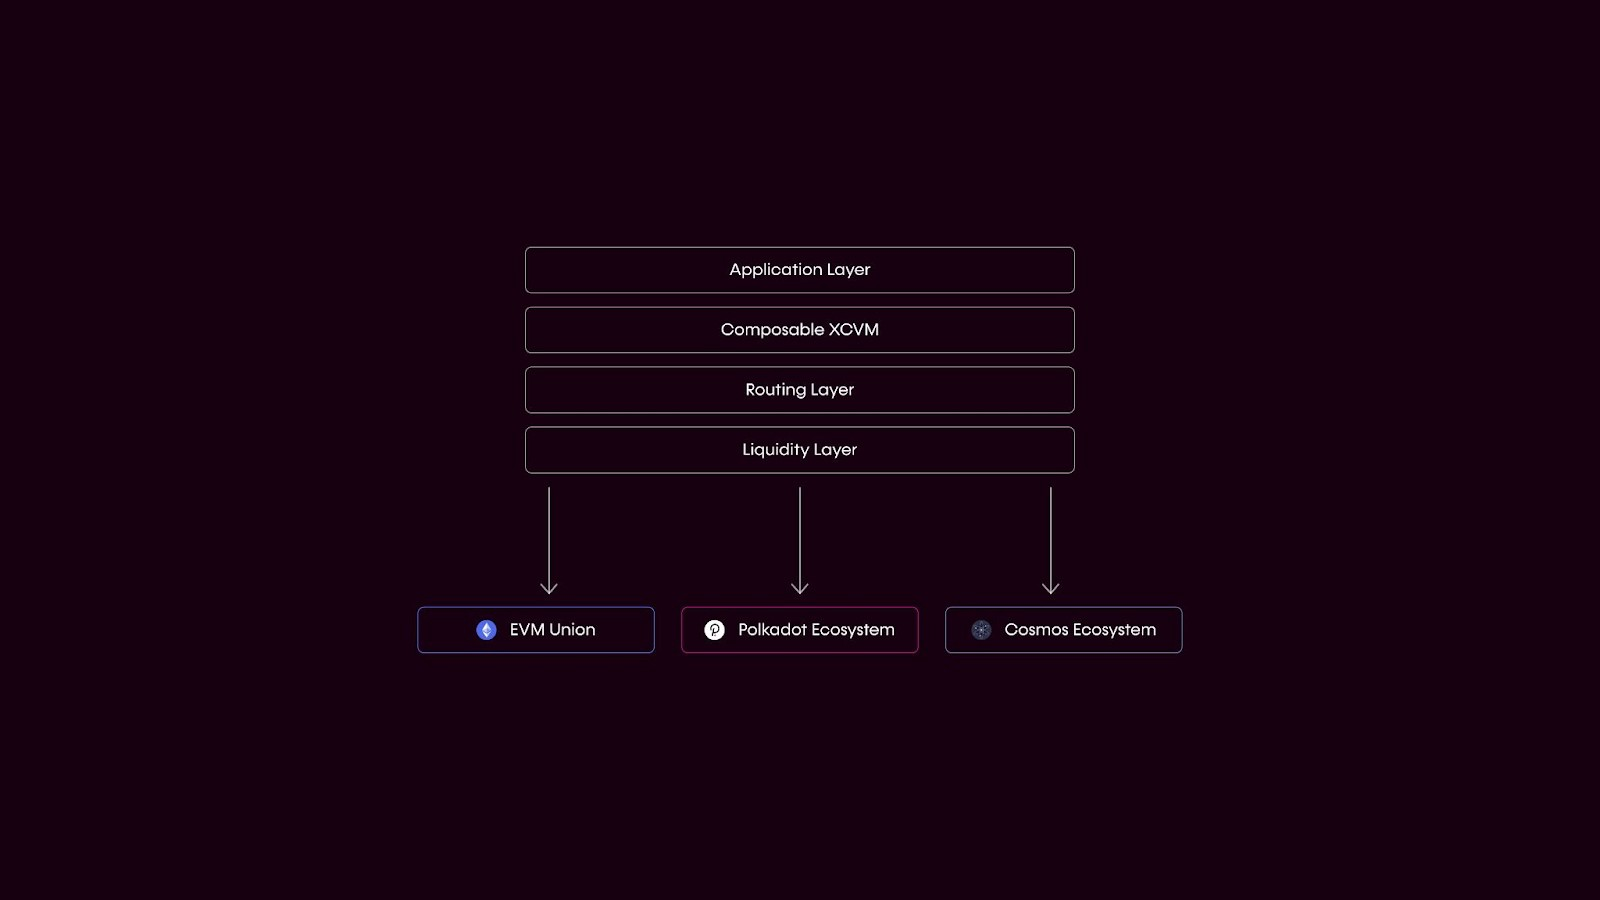
\includegraphics[width=15cm]{images/stack.jpg}
    \caption{Composable Finance's architecture.}
    \label{fig:stack}
\end{figure}
%

\subsection{Cross chain virtual machine (XCVM)}

The Composable XCVM allows for cross-ecosystem communication. We conceptualize this in Fig.~(\ref{fig:xcvm}) and it provides a single developer-friendly interface to orchestrate the interaction with different bridges, manage routing, initiate callbacks into smart contracts, reliability, and finality. Our Mosaic ecosystem will leverage this virtual machine to facilitate the asset transfers, which allow cross-chain transactions and support parachain-L2 connections. Economic stakes guarantee the security of this system through fraud-proofs and disputes.
%
\begin{figure}
    \centering
    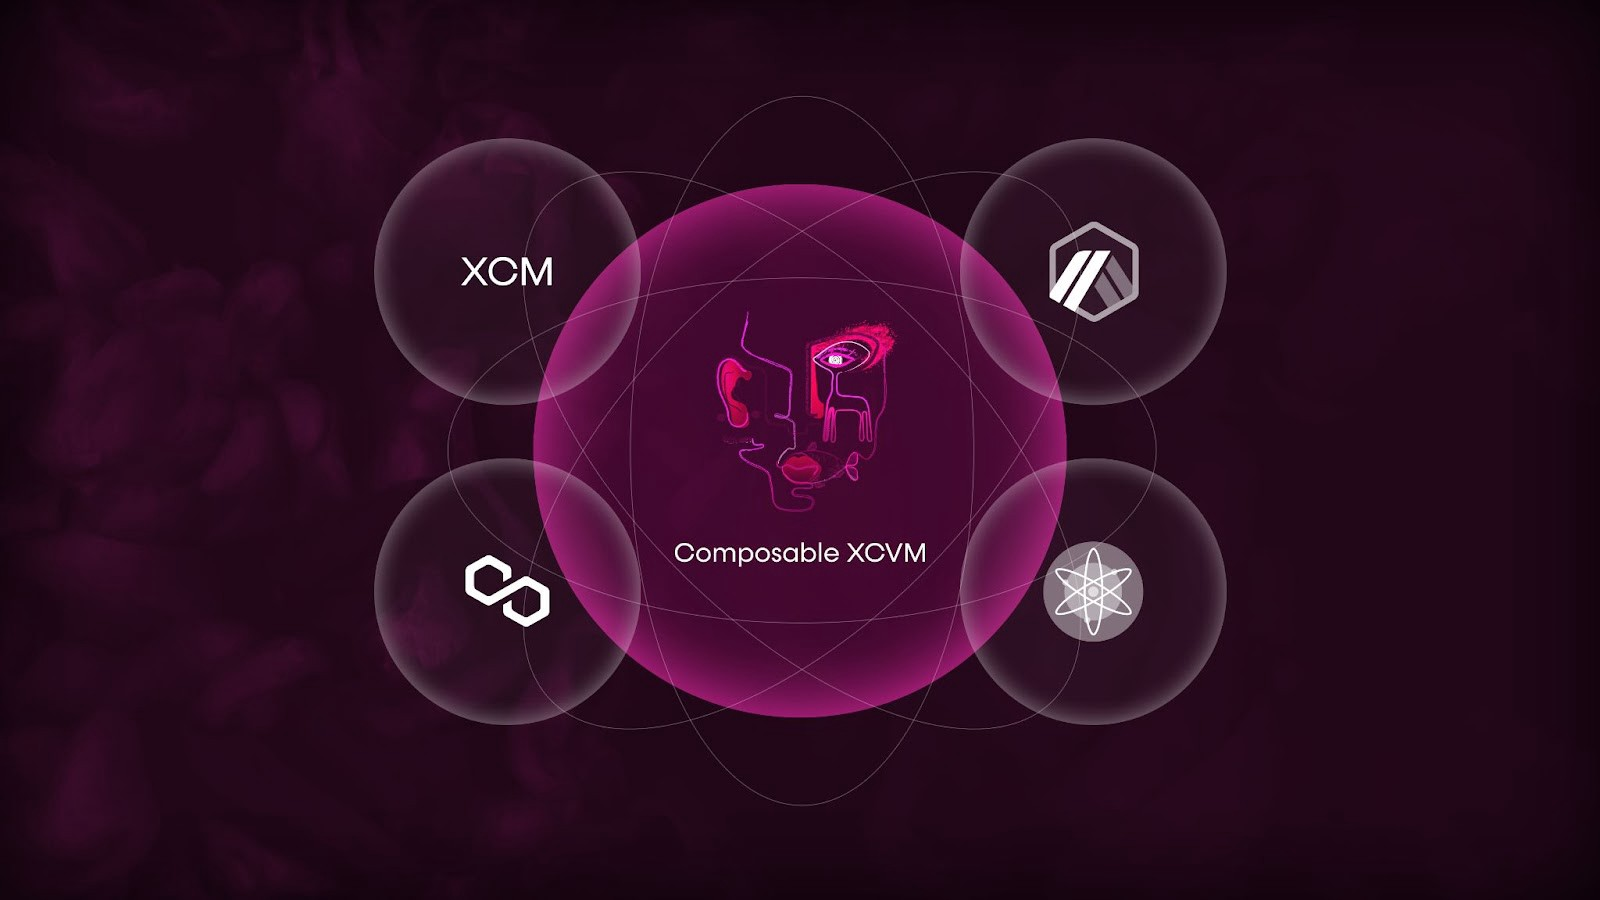
\includegraphics[width=15cm]{images/xcvm.jpg}
    \caption{Composable Finance's Cross-Chain Virtual Machine (XCVM).}
    \label{fig:xcvm}
\end{figure}
%
In order to facilitate this communication, we need two specific components that we are currently building: the Communication and Finality layers of our XCVM.

The idea of our solution , however, is not to create a new standard for cross-chain communication, which is already the object of a number of projects. Instead, the intention is to serve as a data availability layer for existing cross-chain communication protocols like IBC and Polkadot’s cross-chain message passing (XCMP).

\subsection{Communication layer/Innovation Availability layer (IAL)}
\begin{itemize}
    \item Polkadot-IBC cross-chain communication and asset transfers
    \item L2-L2 communication and transfers through our parachain
\end{itemize}
    
\subsection{Finality layer}
\begin{itemize}
        \item Our parachain offering is Picasso on Kusama, and name to be determined on Polkadot.
\end{itemize}

\subsection{Routing Layer}

Incentivized pathway selection to allow for users to perform actions, in an ecosystem agnostic manner.

Our Routing Layer will assess all of the possibilities for a given action (i.e. taking out a loan of 1000 USDC) across all potential layers and chains, and selects the optimal pathway for a user. This layer will be crypto-economically secured, with incentives provided for actors to properly select the best routes for user actions. Thus, this will act as a function aggregator, providing optimal services to users without them having to scour the entire expanse of the DeFi space themselves for the most promising opportunities and best deals.

One exciting application for this pathway execution layer is in cross-chain fee management. Our infrastructure as a whole intends to support a network of blockchain networks, meaning that there will be multiple potential pathways to the same destination. In this scenario, without a tool to do so for them, users would have to pathfind the most efficient and compliant route for value packets. Users may need to prioritize efficiency if the pathway must be especially liquid or secure, or if a specific regulatory requirement must be enforced (such as know your customer/anti-money laundering requirements, abbreviated KYC/AML). Therefore, the routing process would be both incredibly important and very time intensive. Our pathway execution layer will make this process simple for users and enable them to customize which parameter they want to optimize for when completing a given transaction.

Upon instruction and orchestration by the Composable Cross-Chain VM,the routing layer selects the most optimal route for the user’s desired outcome, which propagates communications cross-ecosystem, and to our to the dApp transport module, Mosaic, which then facilitates asset transfers, with settlement being recognized on the parachain.

\subsection{Mosaic: The liquidity infrastructure layer}

Mosaic (the liquidity layer that communicates with Composable XCVM and the Routing Layer), serves to ensure liquidity is moving to the locations where it is needed, allowing the propagation of whatever instructions are required to satisfy the user’s desired outcome, as specified above. We are currently testing this capacity within the EVM ecosystem by running our Proof of Concept (PoC) of Mosaic. From there, we can generalize this liquidity problem and solution to other ecosystems.

Liquidity concerns are not new in DeFi. However, they have largely been resolved by automated market makers (AMMs) built into the popular DeFi exchanges like UniSwap and Sushiswap. The introduction of cross-layer and cross-chain applications is, however, making liquidity a more pressing issue than ever before; with so many different layer 2 applications and blockchains to balance liquidity across, and so little infrastructure to do so, liquidity is very siloed for interoperable applications.

Composable Labs has built a Liquidity Simulation Environment (LSE) to better explore the opportunity and best means of cross-layer liquidity provisioning (LPing). The first phase of this experimentation was to determine the viability of cross-layer liquidity provisioning by running test trade data through our model. This resulted in the prediction that LPs could be positioned to earn an impressive 16\% return per week for providing liquidity for cross-L2 transfers. The second phase of this experiment is underway, wherein we have deployed our PoC of our cross-layer asset transferral system Mosaic, with the PoC being our Polygon-Arbitrum Cross-Layer Transferral System, to test out the associated dynamic fee model. Once we have scraped this data, we will be able to prove out the dynamic fee model and, as a broader goal, our passive liquidity provider role in this system. This data will also assist us with the rebalancing work I have recently released as well.

Lastly, our full solution will have an active management model as I have previously indicated as well. These bots will be working to reorganize transactions in a manner that maximizes fees, ensuring that trades are able to go through.

With this full model, we hope to generalize the model for meeting liquidity demands for cross-chain transfers. Initially, we are focused on the EVM universe, but will expand this vision for Mosaic to deliver the infrastructure needed for developers to create any of an infinite number of cross-layer dApps and have appropriate liquidity be available to their users.

Following this progress with the EVM, we want to expand from ensuring cross-layer liquidity on Ethereum to ensuring cross-layer liquidity on other chains as well; there are still cross-layer liquidity problems within the Inter Blockchain Communication (IBC) Protocol, Cosmos SDK chains, and Polkadot. We aspire to create a continual flow of liquidity between all of these ecosystems.
